\section{Realisierung}

\subsection{Allgemeines}

\subsubsection{Timeouts}

In der Implementierung ist, bis auf Ausnahmen, für jeden \textit{receive} Block ein \textit{Timeout} eingebaut. Dieser beträgt 1000ms. Wird der Timeout ausgelöst, wird eine für jeden Fall individuelle Fehlermeldung geloggt.

\subsubsection{Responses}

Um die jeweiligen Nachrichten und vor allem die Responses korrekt einordnen zu können, sind diese wie folgt aufgebaut:\\
Wird die Nachricht $\{self(), \{getMessage\}\}$ an den \textit{Prozess der Kommunikationseinheit} geschickt, dann ist die Antwort: $\{replycbcast, ok\_getMessage, \{...\}\}$. Anhand folgender Tabelle \ref{tab:namenszuordnung} kann eine Antwort-Nachricht eindeutig zugeordnet werden.

\begin{table}[h]
    \centering
    \begin{tabular}{|c|c|}
        \hline
        TowerClock & replyclock \\
        \hline
        TowerCBC & replycbc \\
        \hline
        Prozess der Kommunikationseinheit & replycbcast \\
        \hline
        Prozess der Queues & replyqueues \\
        \hline
    \end{tabular}
    \caption{Namenszuordnung}
    \label{tab:namenszuordnung}
\end{table}
\subsection{Kommunikationseinheit}

\subsubsection{init/0} \label{cbcast_init_realisierung}

Die Initialisierung der \textit{Kommunikationseinheit} erzeugt einen Prozess, dessen Prozess ID zurückgegeben wird.
Wie in Abb. \ref{fig:sequence_cbCast_cbcast} zu sehen muss erst eine Verbindung zum \textit{Tower} hergestellt werden. Über die \textit{erlang} Funktion \textit{net\_adm:ping/1} wird angefragt, ob die \textit{Node} des \textit{Towers} erreichbar ist. Anschließend wird der eigentlich Prozess gestartet, diesem werden zuerst die Datei, in welcher geloggt wird und die Adresse des \textit{Towers} mitgebenen.\\Aus dem neuen Prozess heraus, werden jetzt zwei wichtige Schritte getriggert:

\paragraph{Die Initialisierung der Vektoruhr} und die anschließenende Erzeugung eines neuen Prozesses für die \textit{Holdback} und \textit{Delivery Queue}, im Folgenden bezeichnet als der \textit{Prozess für die Queues}. Folgende Funktion zeigt die gespeicherten Zustände dieses Prozesses und die verfügbaren Schnittstellen.

\begin{lstlisting}
loopQueues(Datei, VT, HBQ, DLQ) ->
    receive
        {From, {pushHBQ, {Message, NewVT}}} ->
            ...
        {From, {pushDLQ, {Message, NewVT}}} ->
            ...
        {From, {popDLQ}} ->
            ...
        {From, {checkQueues}} ->
            ...
        {From, {syncVT, {AsyncVT}}} ->
            ...
        {From, {tickVT}} -> 
            ...
        {From, {getVTid}} ->
            ...
        {From, {listQueues}} ->
            ...
        Any -> 
            ...
    end.
\end{lstlisting}

Der Prozess speichert die Datei, in welcher geloggt wird als Zeichenkette, den Vektorzeitstempel in der in Kapitel \ref{vectorC_realisierung} festgelegten Datenstruktur und die \textit{Holdback} und \textit{Delivery} Queue jeweils als Liste. Während \textit{listQueues} nur eine convenience Schnittstelle ist, welche ausschließlich zum Debuggen genutzt wird, haben alle anderen Schnittstellen eine wichtige Funktionalität: 
\begin{itemize}
    \item \textit{pushHBQ} und \textit{pushDLQ} fügen Nachrichten der jeweiligen \textit{Queue} hinzu
    \item \textit{popDLQ} entfernt eine Nachricht nach dem FiFo Prinzip aus der \textit{Delivery Queue}
    \item \textit{checkQueues} (siehe Abb. \ref{fig:flow_checkQueues}) prüft ob in der \textit{Holdback Queue} auslieferbare Nachrichten enthalten sind und sortiert diese entsprechend in die \textit{Delivery Queue}
    \item \textit{syncVT} synchronisiert die im Prozess gespeicherte Vektoruhr mit einer als Parameter mitgelieferten Vektoruhr
    \item \textit{tickVT} erhöht die im Prozess gespeicherte Vektoruhr um 1
    \item \textit{getVTid} gibt die eigene Identität der im Prozess gespeicherten Vektoruhr zurück. 
\end{itemize}

\begin{figure}[htbp]
\begin{center}
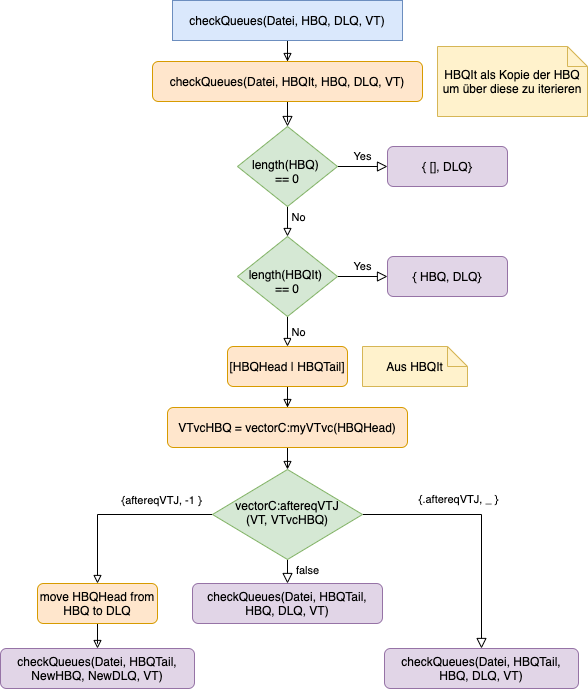
\includegraphics[scale=0.6]{Latex/Bilder/checkQueues.png}
\caption{\label{fig:flow_checkQueues} checkQueues}
\end{center}
\end{figure}
    
\paragraph{Das Empfangen von Nachrichten der Kommunikationseinheit} was das Senden und das blockierende und nicht blockierende Empfangen von Nachrichten vom und an den \textit{Tower} ermöglicht. Dieser Prozess speichert die in die zu loggende Datei, die Adresse des \textit{Towers} und die Adresse des Prozesses in welchem die \textit{Queues} gespeichert sind. Im Folgenden ist dies der \textit{Prozess der Kommunikationseinheit}.

\begin{lstlisting}
loop(Datei, TowerCBC, Queues) ->
    receive
        {_From, {castMessage, {Message, NewVT}}} ->
            ...
            loop(Datei, TowerCBC, Queues);
        ...
    end.
\end{lstlisting}

\subsubsection{stop/1} \label{cbcast_stop_realisierung}

Wie bereits in Kapitel \ref{commModule_stop} beschrieben, wird das Stoppen zuerst durch einen \textit{Graceful Shutdown} versucht. Dieser schickt eine Nachricht an den Prozess nach dessen Bearbeitung dieser sich selbst nicht wieder aufruft und somit terminiert. Schlägt dies fehl, wird nach einem Timeout die \textit{erlang} Funktion \textit{exit/2} aufgerufen und ein \textit{Hard Shutdown} durchgeführt.

\subsubsection{send/2} \label{cbcast_send_realisierung}

Versendet wird eine Nachricht indem diese an den \textit{Prozess der Kommunikationseinheit} (\textit{cbCast Prozess}) geschickt wird (siehe Abb. \ref{fig:sequence_send_realisierung}).

\begin{figure}[htbp]
\begin{center}
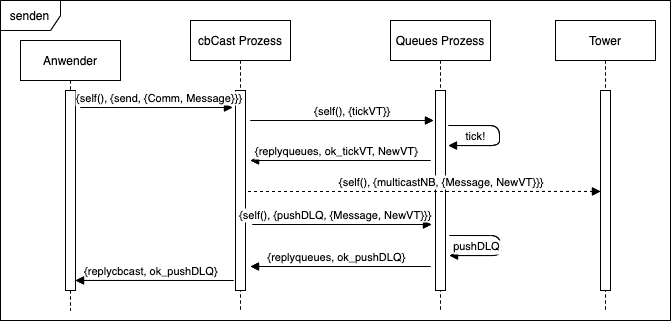
\includegraphics[scale=0.6]{Latex/Bilder/send_realisierung.png}
\caption{\label{fig:sequence_send_realisierung} send/2}
\end{center}
\end{figure}

\subsubsection{read/1 \& received/1} \label{cbcast_read_received_realisierung}

Um eine Nachricht auszuliefern wird auch hier der \textit{Prozess der Kommunikationseinheit} (\textit{cbCast Prozess}) angesprochen. Beide Arten der Auslieferung schicken an die gleiche Schnittstelle. Diese fragt dann über den mitgeschickten Parameter \textit{Blocking} ab ob blockierend oder nicht blockierend ausgeliefert werden soll.

\paragraph{read/1 (nicht blockierend)}

Das nicht blockierende Ausliefern schickt die Nachricht $\{self(), \{getMessage, false\}\}$ (siehe Abb. \ref{fig:sequence_read_realisierung}).

\begin{figure}[htbp]
\begin{center}
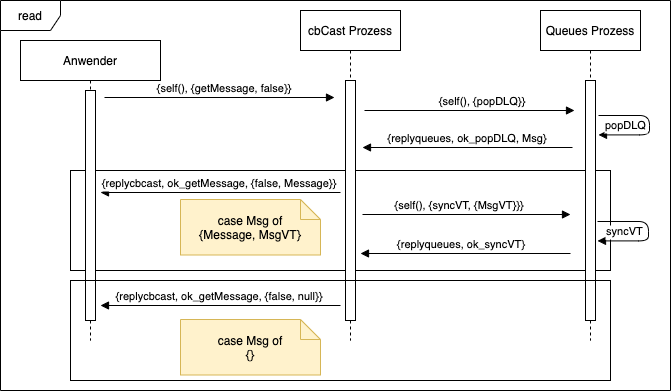
\includegraphics[scale=0.6]{Latex/Bilder/read_realisierung.png}
\caption{\label{fig:sequence_read_realisierung} read/2}
\end{center}
\end{figure}

\paragraph{received/1 (blockierend)}

Das blockierende Ausliefern schickt die Nachricht \\$\{self(), \{getMessage, true\}\}$ (siehe Abb. \ref{fig:sequence_received_realisierung}).

\begin{figure}[htbp]
\begin{center}
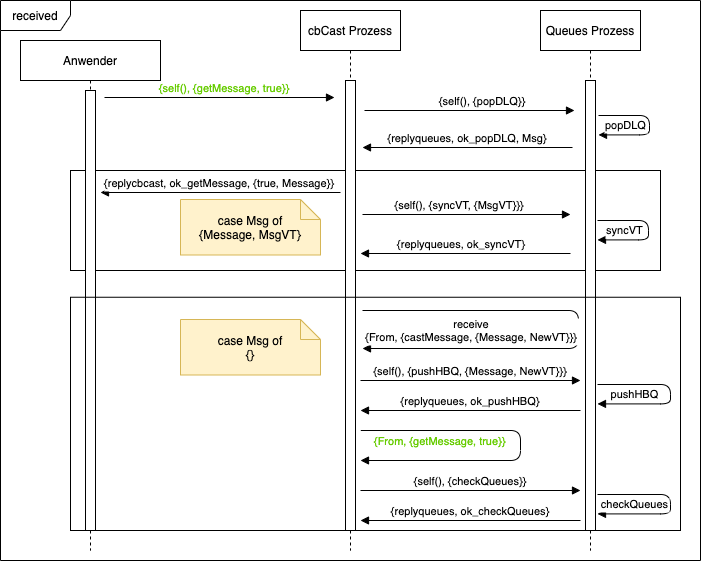
\includegraphics[scale=0.6]{Latex/Bilder/receive_realisierung.png}
\caption{\label{fig:sequence_received_realisierung} received/2}
\end{center}
\end{figure}

\subsubsection{$\{\langle PID \rangle,\{castMessage,\{\langle Message \rangle, \langle VT \rangle\}\}\}$}

Die Schnittstelle \textit{castMessage} (siehe Abb. \ref{fig:sequence_cast_realisierung}) überprüft nach dem Empfangen einer Nachricht ob die Identität der Vektoruhr der Nachricht, die gleiche Identität hat, wie der \textit{Prozess der Kommunikationseinheit}. Wenn dies der Fall ist, wird die Nachricht verworfen, da die Nachricht bereits beim Versenden in der \textit{Delivery Queue} gespeichert wurde.

\begin{figure}[htbp]
\begin{center}
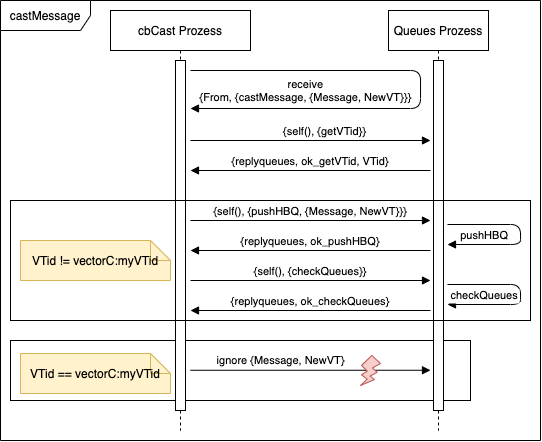
\includegraphics[scale=0.6]{Latex/Bilder/cast_realisierung.png}
\caption{\label{fig:sequence_cast_realisierung} $\{\langle PID \rangle,\{castMessage,\{\langle Message \rangle, \langle VT \rangle\}\}\}$}
\end{center}
\end{figure}

\subsection{Vektoruhr-ADT} \label{vectorC_realisierung}

Die bereits in Kapitel \ref{vectorC_entwurf} beschriebene Datenstruktur ist ein \textit{erlang} Tupel bestehend aus der Vektoruhr Identität als Integer und der Vektoruhr als \textit{erlang} Liste. In der Vektoruhr sind alle Zeitstempel der verschieden \textit{Prozesse der Kommunikationseinheiten}, inklusive dem Eigenen, gespeichert. Als Beispiel: $\{2, [1,3,4,2]\}$. Die Vektoruhr Identität ist $2$ und die Vektoruhr ist $[1,3,4,2]$. Die Identitäten beginnen bei 1. Somit ist der eigene Zeitstempel dieser ADT $3$.

\begin{lstlisting}
VT = {2, [1,3,4,2]}.
vectorC:myCount(VT).
3
\end{lstlisting}

\subsubsection{initVT/0}

Diese Funktion stellt im ersten Schritt eine Verbindung zur \textit{TowerClock} über die \textit{erlang} Funktion \textit{net\_adm:ping/1} her. Ist der Verbindungsaufbau erfolgreich, wird am \textit{TowerClock} die Identität angefragt. Zurückgegeben wird diese Identität \textit{VecID} als Tupel \textit{\{VecID, zeros(VecID)\}}. \textit{zeros/1} erstellt eine Liste, welche genau so viele Nullen enthält, wie es im Parameter übergeben wurde.

\subsubsection{myCount/1}

Über die Hilfsfunktion \textit{getElementByIndex(VT, VTID)} kann der entsprechende Ereigniszähler, bzw. der eigene Zeitstempel gefunden werden.

\subsubsection{foCount/2}

\textit{foCount/2} wirft eine Exception, wenn die übergebene Position J kleiner als 0 oder größer als die Länge der verfügbaren Zeitstempel ist.

\begin{lstlisting}
foCount(J, {_VTID, VT}) when J > 0 andalso J =< length(VT)-> getElementByIndex(VT, J);
foCount(_, _) -> throw({error, "Invalid index. Index must be greater than 0 and smaller than the size of available timestamps."}).
\end{lstlisting}

\subsubsection{isVT/1}

Zuerst wird geprüft ob das Tupel genau zwei Elemente enthält. Trifft dies zu, wird geprüft, dass
\begin{enumerate}
    \item das erste Element ein Integer ist,
    \item das zweite Element eine Liste ist,
    \item jedes Element der Liste ein Integer ist.
\end{enumerate}

\subsubsection{syncVT/2} \label{syncVT_realisierung}

Im ersten Schritt dieser Funktion wird zuerst die Länge der beiden übergebenen Vektoruhren anhand der Hilfsfunktion \textit{padWithZeros/2} normalisiert:

\begin{lstlisting}
NormalizedVT1 = padWithZeros(VT1, length(VT2)),
NormalizedVT2 = padWithZeros(VT2, length(VT1)),
\end{lstlisting}

Diese beiden Vektoruhren werden dann Index für Index miteinander verglichen. Es wird jeweils das Maximum der beiden Werte als neue Liste gespeichert und zusammen mit der Identität der ersten Vektoruhr zurückgegeben.

\subsubsection{tickVT/1}

\textit{tickVT/1} nutzt die Hilfsfunktion \textit{incrementElementAtIndex/3}. Übergeben werden dieser Funktion die Vektoruhr an sich, die Identität und ein Counter.

\subsubsection{compVT/2}

Auch in \textit{compVT/2} werden zuerst die beiden Vektoruhren normalisiert (siehe Kapitel \ref{syncVT_realisierung}). 
Anschließend wird die Hilfsfunktion \textit{compareLists/3} (siehe Abb. \ref{fig:flow_compVT_realisierung}) aufgerufen.

\begin{figure}[htbp]
\begin{center}
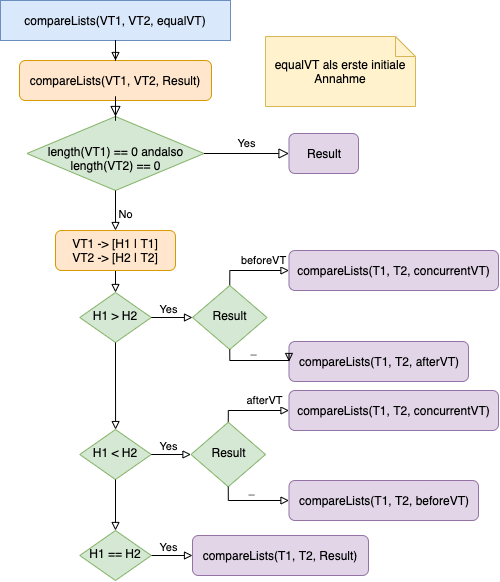
\includegraphics[scale=0.6]{Latex/Bilder/compVT_realisierung.png}
\caption{\label{fig:flow_compVT_realisierung} compVT}
\end{center}
\end{figure}

\subsubsection{aftereqVTJ/2}

Die Funktion \textit{aftereqVTJ/2} (siehe Abb. \ref{fig:flow_aftereqvtj_realisierung}) nutzt zwei weitere Funktionen. Zuerst die \textit{removeJ/2} Hilfsfunktion, welche in beiden Vektoruhren ein Element entfernt und dann die beiden neuen Vektoruhren vergleicht (siehe Kapitel \ref{aftereqvtj_entwurf}).

\begin{figure}[htbp]
\begin{center}
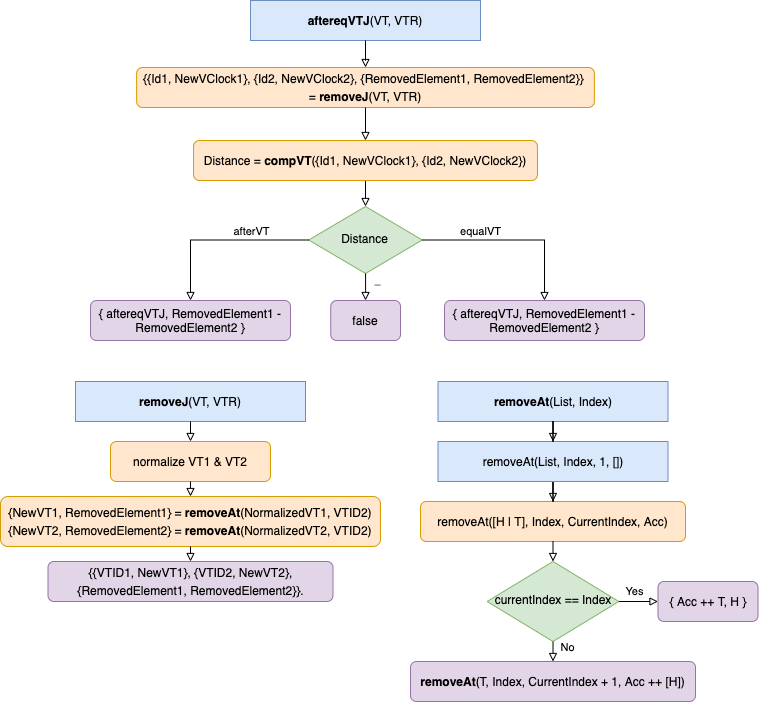
\includegraphics[scale=0.55]{Latex/Bilder/aftereqVTJ_realisierung.png}
\caption{\label{fig:flow_aftereqvtj_realisierung} aftereqVTJ/2}
\end{center}
\end{figure}

\subsection{Ungeordneter Multicast}

\subsubsection{init/1}

Wie bereits in Kapitel \ref{towercbc_init_entwurf} beschrieben, kann der \textit{Tower} in zwei verschiedenen Modi gestartet werden. Diese werden dem Prozess in der Booleschen Variable \textit{Auto} übergeben. Der Prozess wird im folgenden als der \textit{Prozess des TowerCBCs} bezeichnet. Wird als Parameter \textit{auto} übergeben, wird die Variable \textit{Auto} auf true gesetzt. Für den Parameter \textit{manu} wird \textit{Auto} als false gespeichert. In der Variable \textit{Registered} werden alle registrierten \textit{Prozesse der Kommunikationseinheiten} gespeichert. Die Variable ist eine Liste nach dem FiFo Prinzip. Dies wird in Kapitel \ref{towercbc_register_realisierung} genauer beschrieben. Auch die letzte Variable \textit{Buffer} ist eine Liste nach dem FiFo Prinzip. In dieser Liste werden alle Nachrichten welche über die Schnittstelle $\{\langle PID\rangle,\{multicastNB,\{\langle Message\rangle,\langle VT\rangle\}\}\}$, beschrieben in Kapitel \ref{towercbc_nb_realisierung}, empfangen werden, gespeichert.

\begin{lstlisting}
loop(Datei, Registered, Auto, Buffer) ->
    receive
        ...
    end.
\end{lstlisting}

\subsubsection{stop/1}

Das Stoppen dieses Prozesses ist identisch zu Kapitel \ref{cbcast_stop_realisierung} umgesetzt.

\subsubsection{listall/0}

Diese Funktion schickt eine Nachricht an den \textit{Prozess des TowerCBCs} welcher daraufhin alle, in der Variable \textit{Registered}, gespeicherten Prozess Ids in die zu loggende Datei schreibt. 

\subsubsection{cbcast/2}

Als Parameter empfängt diese Funktion zwei Integer, welche zuerst auf den richtigen Datentypen geprüft werden. Die Parameter sind Indexe für die beiden Listen, welche im \textit{Prozess des TowerCBCs} gespeichert sind. Um sicherzustellen, dass diese Indexe mindestens größer als 0 sind ist diese Bedingung als Guard in der Funktion integriert. Anschließend wird eine Nachricht an den \textit{Prozess des TowerCBCs} geschickt. Diese ist in Kapitel \ref{towercbc_m_realisierung} aufgeführt.

\subsubsection{$\{\langle PID \rangle,\{register,\langle RPID\rangle\}\}$} \label{towercbc_register_realisierung}

Beim Senden an diese Schnittstelle wird über die Hilfsfunktion \textit{isListMember/2} geprüft ob die mitgeschickte Prozess ID \textit{RPID} bereits in der Liste \textit{Registered} enthalten ist. Ist dies der Fall, ist die Antwort an den Sender der Nachricht $\{replycbc, ok\_existing\}$. Wenn nicht, dann wird die Prozess ID der Liste hinzugefügt und die Antwort ist $\{replycbc, ok\_registered\}$.

\subsubsection{$\{\langle PID\rangle,\{multicastB,\{\langle Message\rangle,\langle VT\rangle\}\}\}$} \label{towercbc_b_realisierung}

Auch bei dieser Schnittstelle wird die Hilfsfunktion \textit{isListMember/2} genutzt um sicherzustellen, dass keine, nicht im \textit{Prozess des TowerCBCs} registrierten Prozesse, Nachrichten via \textit{Multicast} verschicken können. Ist die Registrierung bestätigt wird die, in der Nachricht mitgeschickte, Vektoruhr über die Funktion \textit{vectorC:isVT/1} auf syntaktische Echtheit geprüft. Ist auch dieser Test bestanden, wird die Nachricht an alle \textit{Prozesse der Kommunikationseinheiten} geschickt, welche in der Liste \textit{Registered} enthalten sind. 

\subsubsection{$\{\langle PID\rangle,\{multicastNB,\{\langle Message\rangle,\langle VT\rangle\}\}\}$} \label{towercbc_nb_realisierung}

Wie bereits in Kapitel \ref{towercbc_init_entwurf} beschrieben, ist diese Schnittstelle nur im \textit{manu} Modus möglich. Die Variable \textit{Auto} muss also auf \textit{false} gesetzt sein. Ähnlich zur vorherigen Schnittstelle (siehe Kapitel \ref{towercbc_b_realisierung}) wird in dieser zuerst der Sender der Nachricht überprüft. Ist dieser Registriert und ist die mitgeschickte Vektoruhr validiert wird die Nachricht an die im \textit{Prozess des TowerCBCs} gespeicherte Liste \textit{Buffer} angehängt.

\subsubsection{$\{\langle PID\rangle,\{multicastM,\langle CommNR\rangle,\langle MessageNR\rangle\}\}$} \label{towercbc_m_realisierung}

Die letzte Schnittstelle wird über \textit{cbcast/2} aufgerufen. Diese Funktion überprüft bereits ob die beiden Indizes \textit{CommNR} und \textit{MessageNR} größer 0 sind. Um Angriffe von außen zu vermeiden, wird diese Prüfung erneut vorgenommen. Zusätzlich kann nun geprüft werden, dass die beiden Indizes nicht größer als die Länge der jeweilig zugehörigen Liste sind. Über die Hilfsfunktion \textit{getElementByIndex/2} werden der entsprechende \textit{Prozess der Kommunikationseinheit} und die entsprechende Nachricht ermittelt. Über einen Guard und Pattern Matching kann in einer Zeile überprüft werden, dass die gefundenen Elemente dem korrekten Datentypen entsprechen (siehe Listing \ref{towercbc_m_realisierung_code} Zeile 4).
Ist der Test erfolgreich wird die Nachricht an den Empfänger geschickt und mit $\{replycbc, ok\_send\}$ geantwortet. Schlägt der Test fehlt wird mit $\{replycbc, error\_send\}$ geantwortet.

\begin{lstlisting}[caption={Codeausschnitt multicastM},captionpos=b, label={towercbc_m_realisierung_code}]
Comm = getElementByIndex(Registered, CommNR - 1), % Receiver Index beginnt bei 0
Result = getElementByIndex(Buffer, MessageNR - 1), % Buffer Index beginnt bei 0
case Result of
    {Message, VT} when is_pid(Comm) -> 
        ...
        From ! {replycbc, ok_send};
    _ -> 
        From ! {replycbc, error_send}
end,
\end{lstlisting}

\subsection{Vektoruhr Zentrale/Tower}

Aufgabe der \textit{Vektoruhr Zentrale} ist, allen \textit{Prozessen der Kommunikationseinheiten} eine eindeutige Identität zu geben. Diese ist vom Typ Integer und startet bei 1.

\subsubsection{init/0}

Diese Funktion erzeugt einen Prozess, welcher unter der Prozess ID \textit{vtKLCclockC} registriert wird. Der erzeugte Prozess sieht wie folgt aus:

\begin{lstlisting}
loop(Datei, Map) ->
    receive
        {getVecID, PID} ->
            ...
            loop(...
        {From, {stop}} when is_pid(From)->
            ...
        Any -> 
            util:logging(Datei, "Unknown message: "++util:to_String(Any)++"\n"),
            loop(Datei, Map)
    end.
\end{lstlisting}

Gespeichert wird einmal die in die zu loggende Datei und eine Map. Die Map ist als Liste implementiert, welche Objekte aus Key Value Paaren enthalten. Die Keys sind Prozess IDs, die Values sind Integer.

\subsubsection{stop/1}

Das Stoppen des Prozesses funktioniert wie in Kapitel \ref{cbcast_stop_realisierung}.

\subsubsection{$\{getVecID,\langle PID\rangle\}$}

Diese Schnittstelle empfängt eine Prozess ID. Anschließend wird überprüft ob in der Map des Prozesses bereits ein Objekt mit einer solchen Prozess ID gespeichert ist. Wenn ja, wird die zugehörige Identität zurückgeschickt. Ansonsten wird eine neue Identität erzeugt, mit der Prozess ID zusammen in der Map gespeichert und zurückgeschickt. Diese neue Identität berechnet sich durch $length(Map) + 1$.

\newpage

\subsection{Anwendung}

Zur Demonstration der korrekten Ausarbeitung wurde eine Anwendung implementiert. Diese liegt in der \textit{app.erl}.
Aufgabe der Anwendung ist, ein Szenario zu demonstrieren (siehe Abb. \ref{seq:entwurf_anwendung}), in welchem zuerst Nachrichten von verschiedenen Nutzern an einen Multicast geschickt werden. Aufgrund eines simulierten Fehlers, werden im Multicast alle Nachrichten in der Reihenfolge vertauscht. Anschließend liest ein dritter Nutzer die Nachrichten aus. Die kausale Ordnung muss bestehen bleiben.

\begin{figure}[htbp]
\begin{center}
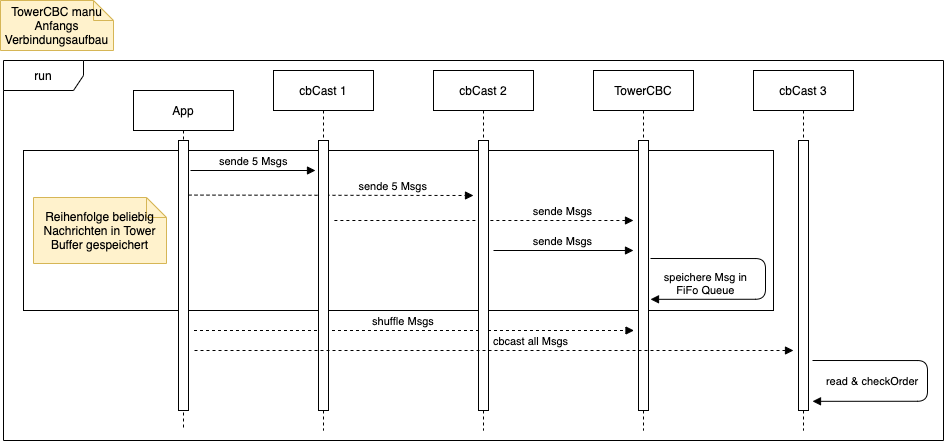
\includegraphics[scale=0.45]{Latex/Bilder/entwurf.png}
\caption{\label{seq:entwurf_anwendung} Entwurf der Anwendung}
\end{center}
\end{figure}

Nach erfolgreicher Ausführung sind folgende Logs (siehe Abb. \ref{logs_anwendung}) zu sehen:

\begin{figure}[htbp]
\begin{center}
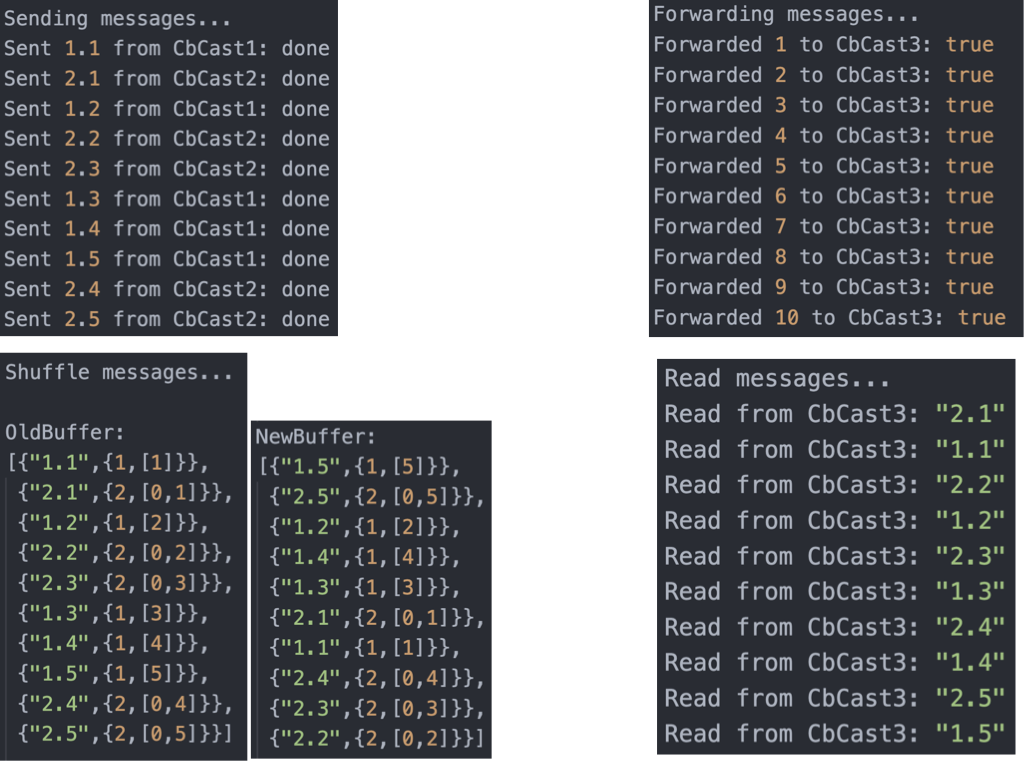
\includegraphics[scale=0.3]{Latex/Bilder/app_log.001.png}
\caption{\label{logs_anwendung} Entwurf der Anwendung}
\end{center}
\end{figure}

Die totale Ordnung ist nicht mehr vorhanden, zum Beispiel ist zuerst die Nachricht '1.1' und dann die Nachricht '2.1' versendet worden. Ausgeliefert wird aber zuerst die '2.1' und dann die '1.1'. Die kausale Ordnung ist aber noch intakt. Die Reihenfolge der von \textit{cbCast1} und \textit{cbCast2} gesendeten Nachrichten stimmt soweit, wenn man diese getrennt voneinander betrachtet. Nach '2.1' folgt '2.2' und nach '1.1' folgt '1.2', usw.. 

\subsubsection{Implementierungsbesonderheiten}

Um die Schnittstellen der jeweiligen Module nicht zu verändern wurden in der \textit{app.erl} verschiedenen Hilfsfunktionen implementiert. 

\paragraph{cbCast}

Das Starten und lokale Registrieren der \textit{Prozesse der Kommunikationseinheiten} erfolgt remote über ein \textit{spawn/2}. Die Hilfsfunktion \textit{startC/1} ist in der \textit{app.erl} implementiert, wird aber auf dem Node des jeweiligen \textit{Prozesses der Kommunikationseinheit} ausgeführt. Somit kann eine lokale Prozess ID erzeugt werden und der Prozess mit einem individuellen Namen registriert werden.

\begin{lstlisting}
% app.erl 

% Verbindungsaufbau
case net_adm:ping(CbCast1Node) of ...

% Erzeugen des Prozesses remote auf dem Node des Comms
spawn(CbCast1Node, fun() -> startC(CbCastName) end)

% Hilfsfunktion um Prozess lokal auf dessen Node zu registrieren
startC(Name) ->
    CommCBC = cbCast:init(),
    erlang:register(Name,CommCBC),
    ...
\end{lstlisting}

\paragraph{towerCBC}

Der \textit{Tower} empfängt für die Anwendung eine zusätzliche Schnittstelle \\$\{From, \{shuffleMessages\}\}$. In dieser werden alle Nachrichten, welche in der Variable \textit{Buffer} gespeichert, sind gemischt. Aufgerufen wird die Schnittstelle vom Prozess der Anwendung aus.

\begin{lstlisting}
% app.erl

Tower ! {{app, erlang:node()}, {shuffleMessages}},
    receive
        {replycbc, ok_shuffleMessages, {OldBuffer, NewBuffer}} -> ...
    after 1000 -> ...
    end.
\end{lstlisting}